\documentclass[border=3pt]{standalone}
% Preâmbulo compartilhado pelos diagramas TikZ da aula 10 (Localização de Markov e Gaussiana)
\usepackage[T1]{fontenc}
\usepackage[utf8]{inputenc}
\usepackage{lmodern}
\usepackage{amsmath}
\usepackage{xcolor}
\usepackage{tikz}
\usetikzlibrary{arrows.meta,angles,quotes,decorations.pathmorphing,calc,
                positioning,shapes.geometric,shapes.misc,backgrounds,fit,
                math}

% Paleta (mesma dos SVGs originais)
\definecolor{dblue}{HTML}{2A5B8C}
\definecolor{dorange}{HTML}{B3541E}
\definecolor{dgreen}{HTML}{4A7C59}
\definecolor{dred}{HTML}{9C4B4B}
\definecolor{dcream}{HTML}{F4F1EA}
\definecolor{dshade}{HTML}{DDD7C9}

% Função gaussiana (não normalizada por padrão de escala visual)
\pgfmathdeclarefunction{gauss}{3}{%
  \pgfmathparse{1/(#3*sqrt(2*pi))*exp(-((#1-#2)^2)/(2*#3^2))}%
}

% Estilos comuns (prefixo d... para não colidir com chaves internas do pgf)
\tikzset{
  >={Stealth[length=2mm]},
  dguide/.style={gray!55, dashed, line width=0.4pt},
  daxis/.style={gray!60, line width=0.7pt, ->},
  dbody/.style={fill=black!3, draw=black!80, line width=1pt},
  dacc/.style={draw=dblue, line width=1pt},
  dlbl/.style={black!55, font=\small},
  dsub/.style={black!45, font=\footnotesize},
  dstate/.style={circle, draw=black!80, fill=dcream, line width=1pt,
                 minimum size=17mm, font=\large, inner sep=1pt},
  dobs/.style={circle, draw=black!80, fill=dshade, line width=1pt,
               minimum size=14mm, font=\large, inner sep=1pt},
  dbox/.style={rounded corners=2pt, draw=black!80, fill=dcream, line width=1pt,
               align=center, inner sep=6pt},
  dop/.style={circle, draw=black!80, fill=white, line width=1pt,
              minimum size=6mm, inner sep=0pt, font=\small},
  dtrans/.style={->, dblue, line width=1pt},
  dmeas/.style={->, dorange, line width=1pt},
  dcurve/.style={line width=1pt, dblue},
  dcurveb/.style={line width=1.4pt, dorange},
}

\usetikzlibrary{shapes.callouts}
\begin{document}
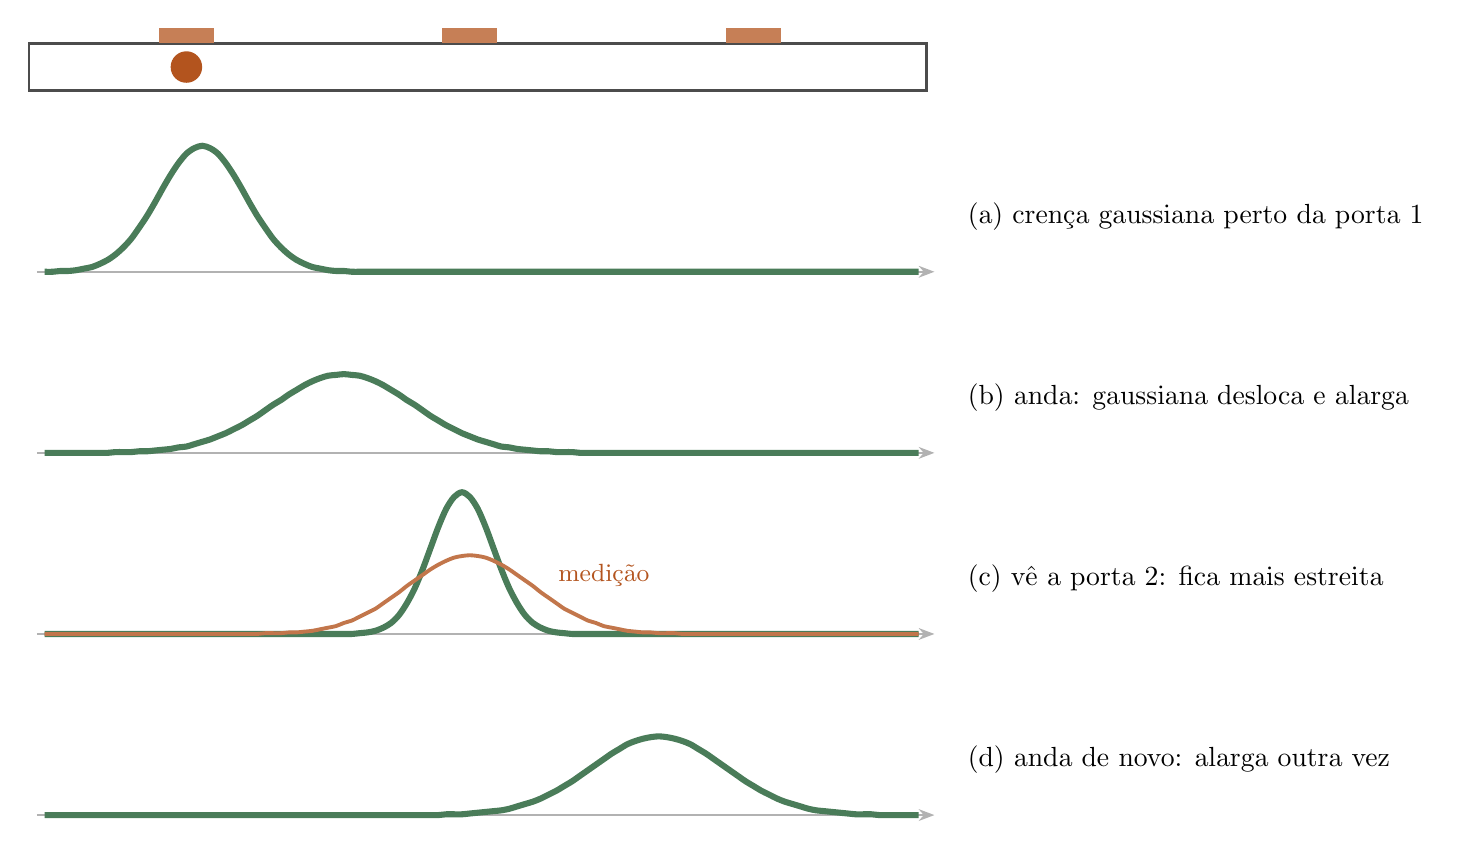
\begin{tikzpicture}[x=1cm,y=1cm,bal/.style={rectangle callout, rounded corners=7pt, draw=black!75, fill=white, line width=1pt, align=center, font=\normalsize, inner sep=5pt}]
\draw[black!70, fill=white, line width=0.9pt] (0,9.70) rectangle (11.4,10.30);
\fill[dorange!75] (1.65,10.30) rectangle (2.35,10.50);
\fill[dorange!75] (5.25,10.30) rectangle (5.95,10.50);
\fill[dorange!75] (8.85,10.30) rectangle (9.55,10.50);
\fill[dorange] (2.00,10.00) circle (0.2);
\draw[daxis] (0.1,7.40) -- (11.5,7.40);
\draw[dgreen, line width=2.2pt] plot[smooth] coordinates {(0.20,7.40) (0.30,7.40) (0.40,7.41) (0.50,7.41) (0.60,7.42) (0.70,7.44) (0.80,7.46) (0.90,7.50) (1.00,7.55) (1.10,7.62) (1.20,7.71) (1.30,7.82) (1.40,7.96) (1.50,8.11) (1.60,8.28) (1.70,8.46) (1.80,8.63) (1.90,8.78) (2.00,8.90) (2.10,8.97) (2.20,9.00) (2.30,8.97) (2.40,8.90) (2.50,8.78) (2.60,8.63) (2.70,8.46) (2.80,8.28) (2.90,8.11) (3.00,7.96) (3.10,7.82) (3.20,7.71) (3.30,7.62) (3.40,7.55) (3.50,7.50) (3.60,7.46) (3.70,7.44) (3.80,7.42) (3.90,7.41) (4.00,7.41) (4.10,7.40) (4.20,7.40) (4.30,7.40) (4.40,7.40) (4.50,7.40) (4.60,7.40) (4.70,7.40) (4.80,7.40) (4.90,7.40) (5.00,7.40) (5.10,7.40) (5.20,7.40) (5.30,7.40) (5.40,7.40) (5.50,7.40) (5.60,7.40) (5.70,7.40) (5.80,7.40) (5.90,7.40) (6.00,7.40) (6.10,7.40) (6.20,7.40) (6.30,7.40) (6.40,7.40) (6.50,7.40) (6.60,7.40) (6.70,7.40) (6.80,7.40) (6.90,7.40) (7.00,7.40) (7.10,7.40) (7.20,7.40) (7.30,7.40) (7.40,7.40) (7.50,7.40) (7.60,7.40) (7.70,7.40) (7.80,7.40) (7.90,7.40) (8.00,7.40) (8.10,7.40) (8.20,7.40) (8.30,7.40) (8.40,7.40) (8.50,7.40) (8.60,7.40) (8.70,7.40) (8.80,7.40) (8.90,7.40) (9.00,7.40) (9.10,7.40) (9.20,7.40) (9.30,7.40) (9.40,7.40) (9.50,7.40) (9.60,7.40) (9.70,7.40) (9.80,7.40) (9.90,7.40) (10.00,7.40) (10.10,7.40) (10.20,7.40) (10.30,7.40) (10.40,7.40) (10.50,7.40) (10.60,7.40) (10.70,7.40) (10.80,7.40) (10.90,7.40) (11.00,7.40) (11.10,7.40) (11.20,7.40) (11.30,7.40)};
\node[font=\normalsize, anchor=west] at (11.8,8.10) {(a) crença gaussiana perto da porta 1};
\draw[daxis] (0.1,5.10) -- (11.5,5.10);
\draw[dgreen, line width=2.2pt] plot[smooth] coordinates {(0.20,5.10) (0.30,5.10) (0.40,5.10) (0.50,5.10) (0.60,5.10) (0.70,5.10) (0.80,5.10) (0.90,5.10) (1.00,5.10) (1.10,5.11) (1.20,5.11) (1.30,5.11) (1.40,5.12) (1.50,5.12) (1.60,5.13) (1.70,5.14) (1.80,5.15) (1.90,5.17) (2.00,5.18) (2.10,5.21) (2.20,5.24) (2.30,5.27) (2.40,5.31) (2.50,5.35) (2.60,5.40) (2.70,5.45) (2.80,5.51) (2.90,5.57) (3.00,5.64) (3.10,5.71) (3.20,5.77) (3.30,5.84) (3.40,5.90) (3.50,5.96) (3.60,6.01) (3.70,6.05) (3.80,6.08) (3.90,6.09) (4.00,6.10) (4.10,6.09) (4.20,6.08) (4.30,6.05) (4.40,6.01) (4.50,5.96) (4.60,5.90) (4.70,5.84) (4.80,5.77) (4.90,5.71) (5.00,5.64) (5.10,5.57) (5.20,5.51) (5.30,5.45) (5.40,5.40) (5.50,5.35) (5.60,5.31) (5.70,5.27) (5.80,5.24) (5.90,5.21) (6.00,5.18) (6.10,5.17) (6.20,5.15) (6.30,5.14) (6.40,5.13) (6.50,5.12) (6.60,5.12) (6.70,5.11) (6.80,5.11) (6.90,5.11) (7.00,5.10) (7.10,5.10) (7.20,5.10) (7.30,5.10) (7.40,5.10) (7.50,5.10) (7.60,5.10) (7.70,5.10) (7.80,5.10) (7.90,5.10) (8.00,5.10) (8.10,5.10) (8.20,5.10) (8.30,5.10) (8.40,5.10) (8.50,5.10) (8.60,5.10) (8.70,5.10) (8.80,5.10) (8.90,5.10) (9.00,5.10) (9.10,5.10) (9.20,5.10) (9.30,5.10) (9.40,5.10) (9.50,5.10) (9.60,5.10) (9.70,5.10) (9.80,5.10) (9.90,5.10) (10.00,5.10) (10.10,5.10) (10.20,5.10) (10.30,5.10) (10.40,5.10) (10.50,5.10) (10.60,5.10) (10.70,5.10) (10.80,5.10) (10.90,5.10) (11.00,5.10) (11.10,5.10) (11.20,5.10) (11.30,5.10)};
\node[font=\normalsize, anchor=west] at (11.8,5.80) {(b) anda: gaussiana desloca e alarga};
\draw[daxis] (0.1,2.80) -- (11.5,2.80);
\draw[dgreen, line width=2.2pt] plot[smooth] coordinates {(0.20,2.80) (0.30,2.80) (0.40,2.80) (0.50,2.80) (0.60,2.80) (0.70,2.80) (0.80,2.80) (0.90,2.80) (1.00,2.80) (1.10,2.80) (1.20,2.80) (1.30,2.80) (1.40,2.80) (1.50,2.80) (1.60,2.80) (1.70,2.80) (1.80,2.80) (1.90,2.80) (2.00,2.80) (2.10,2.80) (2.20,2.80) (2.30,2.80) (2.40,2.80) (2.50,2.80) (2.60,2.80) (2.70,2.80) (2.80,2.80) (2.90,2.80) (3.00,2.80) (3.10,2.80) (3.20,2.80) (3.30,2.80) (3.40,2.80) (3.50,2.80) (3.60,2.80) (3.70,2.80) (3.80,2.80) (3.90,2.80) (4.00,2.80) (4.10,2.80) (4.20,2.81) (4.30,2.82) (4.40,2.84) (4.50,2.88) (4.60,2.94) (4.70,3.04) (4.80,3.19) (4.90,3.38) (5.00,3.62) (5.10,3.89) (5.20,4.16) (5.30,4.39) (5.40,4.54) (5.50,4.60) (5.60,4.54) (5.70,4.39) (5.80,4.16) (5.90,3.89) (6.00,3.62) (6.10,3.38) (6.20,3.19) (6.30,3.04) (6.40,2.94) (6.50,2.88) (6.60,2.84) (6.70,2.82) (6.80,2.81) (6.90,2.80) (7.00,2.80) (7.10,2.80) (7.20,2.80) (7.30,2.80) (7.40,2.80) (7.50,2.80) (7.60,2.80) (7.70,2.80) (7.80,2.80) (7.90,2.80) (8.00,2.80) (8.10,2.80) (8.20,2.80) (8.30,2.80) (8.40,2.80) (8.50,2.80) (8.60,2.80) (8.70,2.80) (8.80,2.80) (8.90,2.80) (9.00,2.80) (9.10,2.80) (9.20,2.80) (9.30,2.80) (9.40,2.80) (9.50,2.80) (9.60,2.80) (9.70,2.80) (9.80,2.80) (9.90,2.80) (10.00,2.80) (10.10,2.80) (10.20,2.80) (10.30,2.80) (10.40,2.80) (10.50,2.80) (10.60,2.80) (10.70,2.80) (10.80,2.80) (10.90,2.80) (11.00,2.80) (11.10,2.80) (11.20,2.80) (11.30,2.80)};
\node[font=\normalsize, anchor=west] at (11.8,3.50) {(c) vê a porta 2: fica mais estreita};
\draw[daxis] (0.1,0.50) -- (11.5,0.50);
\draw[dgreen, line width=2.2pt] plot[smooth] coordinates {(0.20,0.50) (0.30,0.50) (0.40,0.50) (0.50,0.50) (0.60,0.50) (0.70,0.50) (0.80,0.50) (0.90,0.50) (1.00,0.50) (1.10,0.50) (1.20,0.50) (1.30,0.50) (1.40,0.50) (1.50,0.50) (1.60,0.50) (1.70,0.50) (1.80,0.50) (1.90,0.50) (2.00,0.50) (2.10,0.50) (2.20,0.50) (2.30,0.50) (2.40,0.50) (2.50,0.50) (2.60,0.50) (2.70,0.50) (2.80,0.50) (2.90,0.50) (3.00,0.50) (3.10,0.50) (3.20,0.50) (3.30,0.50) (3.40,0.50) (3.50,0.50) (3.60,0.50) (3.70,0.50) (3.80,0.50) (3.90,0.50) (4.00,0.50) (4.10,0.50) (4.20,0.50) (4.30,0.50) (4.40,0.50) (4.50,0.50) (4.60,0.50) (4.70,0.50) (4.80,0.50) (4.90,0.50) (5.00,0.50) (5.10,0.50) (5.20,0.50) (5.30,0.51) (5.40,0.51) (5.50,0.51) (5.60,0.52) (5.70,0.53) (5.80,0.54) (5.90,0.55) (6.00,0.56) (6.10,0.58) (6.20,0.61) (6.30,0.64) (6.40,0.67) (6.50,0.71) (6.60,0.76) (6.70,0.81) (6.80,0.87) (6.90,0.93) (7.00,1.00) (7.10,1.07) (7.20,1.14) (7.30,1.21) (7.40,1.28) (7.50,1.34) (7.60,1.40) (7.70,1.44) (7.80,1.47) (7.90,1.49) (8.00,1.50) (8.10,1.49) (8.20,1.47) (8.30,1.44) (8.40,1.40) (8.50,1.34) (8.60,1.28) (8.70,1.21) (8.80,1.14) (8.90,1.07) (9.00,1.00) (9.10,0.93) (9.20,0.87) (9.30,0.81) (9.40,0.76) (9.50,0.71) (9.60,0.67) (9.70,0.64) (9.80,0.61) (9.90,0.58) (10.00,0.56) (10.10,0.55) (10.20,0.54) (10.30,0.53) (10.40,0.52) (10.50,0.51) (10.60,0.51) (10.70,0.51) (10.80,0.50) (10.90,0.50) (11.00,0.50) (11.10,0.50) (11.20,0.50) (11.30,0.50)};
\node[font=\normalsize, anchor=west] at (11.8,1.20) {(d) anda de novo: alarga outra vez};
\draw[dorange!80, line width=1.4pt] plot[smooth] coordinates {(0.20,2.80) (0.30,2.80) (0.40,2.80) (0.50,2.80) (0.60,2.80) (0.70,2.80) (0.80,2.80) (0.90,2.80) (1.00,2.80) (1.10,2.80) (1.20,2.80) (1.30,2.80) (1.40,2.80) (1.50,2.80) (1.60,2.80) (1.70,2.80) (1.80,2.80) (1.90,2.80) (2.00,2.80) (2.10,2.80) (2.20,2.80) (2.30,2.80) (2.40,2.80) (2.50,2.80) (2.60,2.80) (2.70,2.80) (2.80,2.80) (2.90,2.80) (3.00,2.81) (3.10,2.81) (3.20,2.81) (3.30,2.82) (3.40,2.82) (3.50,2.83) (3.60,2.84) (3.70,2.86) (3.80,2.88) (3.90,2.90) (4.00,2.94) (4.10,2.97) (4.20,3.02) (4.30,3.07) (4.40,3.12) (4.50,3.19) (4.60,3.26) (4.70,3.33) (4.80,3.41) (4.90,3.48) (5.00,3.55) (5.10,3.62) (5.20,3.68) (5.30,3.73) (5.40,3.77) (5.50,3.79) (5.60,3.80) (5.70,3.79) (5.80,3.77) (5.90,3.73) (6.00,3.68) (6.10,3.62) (6.20,3.55) (6.30,3.48) (6.40,3.41) (6.50,3.33) (6.60,3.26) (6.70,3.19) (6.80,3.12) (6.90,3.07) (7.00,3.02) (7.10,2.97) (7.20,2.94) (7.30,2.90) (7.40,2.88) (7.50,2.86) (7.60,2.84) (7.70,2.83) (7.80,2.82) (7.90,2.82) (8.00,2.81) (8.10,2.81) (8.20,2.81) (8.30,2.80) (8.40,2.80) (8.50,2.80) (8.60,2.80) (8.70,2.80) (8.80,2.80) (8.90,2.80) (9.00,2.80) (9.10,2.80) (9.20,2.80) (9.30,2.80) (9.40,2.80) (9.50,2.80) (9.60,2.80) (9.70,2.80) (9.80,2.80) (9.90,2.80) (10.00,2.80) (10.10,2.80) (10.20,2.80) (10.30,2.80) (10.40,2.80) (10.50,2.80) (10.60,2.80) (10.70,2.80) (10.80,2.80) (10.90,2.80) (11.00,2.80) (11.10,2.80) (11.20,2.80) (11.30,2.80)};
\node[dorange, font=\small, anchor=west] at (6.6,3.55) {medição};
\end{tikzpicture}
\end{document}
